% !TeX spellcheck = it_IT
\newpage
\section{Probabilità e indipendenza}
Molte decisioni sono prese in condizioni di incertezza. Questo perché non è possibile conoscere con certezza il futuro in quanto qualsiasi affermazione possiamo fare potrebbe avverarsi come no. La teoria della probabilità nasce per quantificare questa incertezza, misurando la fiducia che un evento possa accadere.
\subsection{Spazi di probabilità}

\begin{definition}[Esperimento aleatorio]
	Un esperimento di cui non si conosce con certezza il risultato.
\end{definition}

\begin{definition}[Esito]
	Un ipotetico risultato di un esperimento aleatorio.
\end{definition}

\begin{definition}[Spazio campionario]
	Lo spazio di probabilità $\Omega$ è l'insieme di tutti gli esiti possibili $\omega$ dell'esperimento. 
\end{definition}

\begin{definition}[Evento]
	Un sottoinsieme dello spazio campionario che rappresenta un'affermazione che possiamo fare sull'esito dell'esperimento. Quando ha un solo elemento si dice \textbf{elementare}. $\Omega$ è un \textbf{evento certo} in quanto sottoinsieme improprio dello spazio campionario mentre $\emptyset$ è un \textbf{evento impossibile}.
\end{definition}

\noindent Consideriamo come esperimento il lancio di un dado:
\begin{equation*}
	A = \{\omega_2,\omega_4,\omega_6\} \qquad B=\{\omega_4,\omega_5,\omega_6\}
\end{equation*}
vediamo la corrispondenza tra le operazioni insiemistiche e logiche:
\begin{table}[h!]
	\centering
	\begin{tabular}{|c|c|c|}
		\hline
		\textbf{Operazione insiemistica} & \textbf{Operazione logica} & \textbf{Esempio} \\
		\hline
		$A \cup B$ & Accade $A$ oppure $B$ & $A \cup B = \{\omega_2, \omega_4, \omega_5,\omega_6\}$ \\
		$A \cap B$ & Accadono $A$ e $B$ & $A \cap B = \{\omega_2, \omega_6\}$\\
		$A^c$ & Non accade $A$ & $A^c = \{\omega_1, \omega_3, \omega_5\}$\\
		$A \setminus B$ & Accade $A$ ma non $B$ & $A \setminus B = A \cap B^c = \{\omega_2\}$\\
		\hline
		\textbf{Relazione insiemistica} & \textbf{Relazione logica} & \textbf{Esempio}\\
		\hline
		$A \subseteq B$ & Se accade $A$ allora accade $B$ & $\{\omega_5\} \subset \{\omega_5, \omega_6\}$\\
		$A \cap B = \emptyset$ & Eventi \textbf{incompatibili} & $C$ esce un numero $<2$ e $B$\\
		\hline
	\end{tabular}
\end{table}

\subsection{Probabilità}
\begin{observation}
	Se due eventi sono incompatibili la probabilità che si realizzi uno qualsiasi dei due è la somma delle probabilità dei singoli eventi.
\end{observation}

\begin{definition}[Probabilità classica]
	Consideriamo uno spazio campionario $\Omega$ relativo ad un esperimento e $A\subseteq\Sigma$ un evento. La probabilità di $A$ è un valore $P(A) \in [0,1]$ che misura il grado di fiducia nell'evento.
	\begin{equation}
		P(A)=\frac{\#\text{casi favorevoli ad }A}{\#\text{casi possibili}} = \frac{\#A}{\#\Omega}
	\end{equation}
	Questa definizione è adatta solo se assumiamo che gli eventi elementari sono ugualmente probabili quindi solo per esperimenti su popolazione reale.
\end{definition}

\begin{definition}[Probabilità frequentista]
	Consideriamo un evento articolato in $n$ prove, nel corso del quale si verificano $k$ eventi elementari $\omega_1, \ldots, \omega_k$ incompatibili ma non equiprobabili.\\
	Supponiamo che $\omega_i$ si sia manifestato $n_i$ volte (frequenza assoluta), allora:
	\begin{equation}
		P(\omega_i) = \lim_{n \to \infty}\frac{n_i}{n}
	\end{equation}
	Questa definizione è adatta ai fenomeni fisici e biologici ma non sempre è possibile effettuare davvero tante prove (anche se oggi si simula). Inoltre non è detto che esista sempre il limite.
\end{definition}

\begin{definition}[Probabilità associativa]
	Dato uno spazio campionario $\Omega$ la probabilità è una funzione $P:\mathbb{P}\to \mathbb{R}$ tale che:
	\begin{itemize}
		\item $0 \leq P(A) \leq 1 \qquad \forall A \subseteq \Omega$
		\item $\mathbb{P}(\Omega)=1$
		\item se $(A_n)_{n=1,2,\ldots}$ è una successione di eventi incompatibili vale l'\textbf{addittività}
		\begin{equation}
			P\bigg(\bigcup_{n=1}^{+\infty}A_n\bigg) = \sum_{n=1}^{+\infty}P(A_n)
		\end{equation}
		e se la successione è infinita
		\begin{equation}
			P\bigg(\bigcup_{n=1}^{N}A_n\bigg) = \sum_{n=1}^{+N}P(A_n)
		\end{equation}
	\end{itemize}
\end{definition}

\begin{note}
	Si dice \textbf{trascurabile} un evento $A$ tale che $\mathbb{P}(A)=0$ e \textbf{quasi certo} un evento $A$ tale che $\mathbb{P}(A)=1$. 
\end{note}

\begin{definition}[Spazio di probabilità]
	La coppia $\Omega, P$ si dice spazio di probabilità.
\end{definition}

\begin{proposition}
	Proprietà della probabilità:
	\begin{itemize}
		\item $\mathbb{P}(A^c)=1-\mathbb{P}(A)$ e di conseguenza $\mathbb{P}(\emptyset)=0$
		\item $B \subseteq A \Longrightarrow \mathbb{P}(A\setminus B)=\mathbb{P}(A) - \mathbb{P}(B)$
		\item $\mathbb{P}(A\cup B)=\mathbb{P}(A)+\mathbb{P}(B)-\mathbb{P}(A \cap B)$
	\end{itemize}
\end{proposition}

\begin{proposition}[Limite di una successione di eventi]
	Data una successione di eventi $A_1, \ldots, A_n, \ldots$, questa può essere:
	\begin{itemize}
		\item \textbf{Crescente}: $A_n \subseteq A_{n+1}$ e quindi $A = \bigcup_{n=1}^{+\infty}A_n = \lim_{n \to  \infty A_n}$
		\item \textbf{Decrescente}: $A_n  \supseteq A_{n+1}$ e quindi $A = \bigcap_{n=1}^{+\infty}A_n = \lim_{n \to  \infty A_n}$
	\end{itemize}
	In entrambi i casi vale:
	\begin{equation}
		\mathbb{P}(A) = \lim_{n \to \infty}\mathbb{P}(A_n)
	\end{equation}
\end{proposition}

\subsection{Modello uniforme}
\begin{definition}[Modello uniforme]
	Definiamo il modello uniforme come lo spazio di probabilità$ (\Omega,P)$ tale che $\Omega$ è finito e ogni esito $\omega\in\Omega$ è equiprobabile, ovvero $P(\{\omega\})$ è la stessa $\forall \omega \in \Omega$.
\end{definition}

\subsubsection{Calcolo combinatorio}
Alcune formule notevoli:
\begin{itemize}
	\item \textbf{Sequenze ordinate con ripetizione} di $k$ numeri da $1$ a $n$: $n^k$
	\item  \textbf{Ordinamenti possibili} di $\{1, \ldots, n\}$: $n!$
	\item \textbf{Sequenze ordinate senza ripetizione} di $k$ numeri di $1, \ldots, n$
	\begin{equation*}
		\frac{n!}{(n-k)!} \quad\quad 0 \leq k \leq n
	\end{equation*}
	\item \textbf{Sottoinsiemi} di $\{1, \ldots, n\}$ formati da $k$ elementi
	\begin{equation*}
		\binom{n}{k} = \frac{n!}{k!(n-k)!} \quad\quad 0 \leq k \leq n
	\end{equation*}
\end{itemize}

\subsection{Probabilità condizionata}
Quando si è a conoscenza della realizzazione di un evento, cambia la valutazione di probabilità di ogni altro evento.
\begin{definition}[Probabilità condizionata]
	Dati due eventi $A, B$ con $B$ non trascurabile ($P(B) \neq 0$), la probabilità condizionata di $A$ rispetto a $B$ è
	\begin{equation}
		\mathbb{P}(A \vert B) = \frac{\mathbb{P}(A \cap B)}{\mathbb{P}(B)}
	\end{equation}
\end{definition}

\begin{observation}
	Fissato $B$ non trascurabile la funzione $A \mapsto P(A\vert B)$ è una probabilità. Non vale il contrario.
\end{observation}

\begin{proposition}[Regola dei prodotti]
	Se l'intersezione di eventi $A_1 \cap \ldots \cap A_{n-1}$ non è trascurabile vale
	\begin{equation}
		\mathbb{P}(A_1 \cap \ldots \cap A_n) = \mathbb{P} (A_1) \cdot \mathbb{P}(A_2 \vert A_1) \cdot \ldots \cdot \mathbb{P}(A_n \vert A_1 \cap \ldots \cap A_{n-1})
	\end{equation}
\end{proposition}

\begin{demostration}
	Vediamo la dimostrazione della regola dei prodotti nel caso con $A$ e $B$. Abbiamo:
	\begin{equation*}
		P(A\vert B)=\frac{P(A \cap B)}{P(B)} \qquad \qquad P(B\vert A)=\frac{P(B\cap A)}{P(A)}
	\end{equation*}
	Però, sapendo che $P(A\cap B) = P(B \cap A) $ possiamo dire che
	\begin{equation*}
		P(A \vert B) \cdot P(B) = P(A\cap B) = P(B\cap A) = P(B \vert A) \cdot P(A)
	\end{equation*}
\end{demostration}

\begin{definition}[Condizionamento ripetuto]
	Se $A_1, \ldots, A_n$ sono $n$ eventi con $A_1 \cap \ldots \cap A_n$ non trascurabili, allora:
	\begin{equation}
		P(A_1 \cap \ldots \cap A_n)=P(A_1) \cdot P(A_2 \vert A_1) \cdot P(A_3 \vert A_1 \cap A_2) \cdot \ldots \cdot P(A_n \vert A_1 \cap \ldots \cap A_{n-1})
	\end{equation}
\end{definition}

\begin{definition}[Sistema di alternative]
	Dato un esperimento con spazio campionario $\Omega$, definiamo il sistema di alternative per quell'esperimento il dato di $B_1, \ldots, B_n$ eventi tali che:
	\begin{itemize}
		\item $B_i \cap B_j = \emptyset \qquad \forall i \neq j$
		\item $\bigcup_{i=1}^n B_i = \Omega$
		\item Ciascun $B_i$ è non trascurabile, ovvero $P(B_i)> 0$
	\end{itemize}
\end{definition}

\begin{theorem}[Formula della probabilità o della fattorizzazione]
	Dato $B_1, \ldots, B_n$ un sistema di alternative, per un qualunque evento $A$ vale
	\begin{equation}
		\mathbb{P}(A) = \sum_{i=1}^{n} P(A \cap B_i)= \sum_{i=1}^{n} \mathbb{P}(A \vert B_i) \mathbb{P}(B_i)
	\end{equation}
\end{theorem}

\begin{theorem}[Formula di Bayes]
	Dati $A$ e $B$ due eventi non trascurabili vale
	\begin{equation}
		\mathbb{P}(B \vert A) = \frac{\mathbb{P}(A \vert B)\mathbb{P}(B)}{\mathbb{P}(A)}
	\end{equation}
	In particolare, se $B_i, \ldots, B_n$ è un sistema di alternative vale
	\begin{equation}
		\mathbb{P}(B_i \vert A) = \frac{\mathbb{P}(A \vert B_i)\mathbb{P}(B_i)}{\sum_{j=1}^{n} \mathbb{P}(A B_j)\mathbb{P}(B_j)}
	\end{equation}
\end{theorem}

\begin{note}
	In pratica il teorema di Bayes server per "invertire" il condizionamento. Tipicamente quando l'evento $A$ è un "osservabile" (e.g. esito test diagnostico) e vogliamo dedurre la probabilità di una possibile "causa" (e.g. paziente sano o malato).
\end{note}

\subsubsection{Rappresentazione ad albero}
In certi casi può essere comoda una rappresentazione ad albero (\textbf{chance tree}), ovvero un diagramma che si può fare dall'alto verso il basso o da sinistra verso destra e che si costruisce come segue:
\begin{enumerate}
	\item Per ogni stadio (nodo) ci sono tanti rami quanti i possibili esiti elementari
	\item Il numero totale di percorsi equivale al numero totale degli esiti possibili
	\item Ad ogni ramo è associata la probabilità corrispondente
\end{enumerate}
\begin{center}
	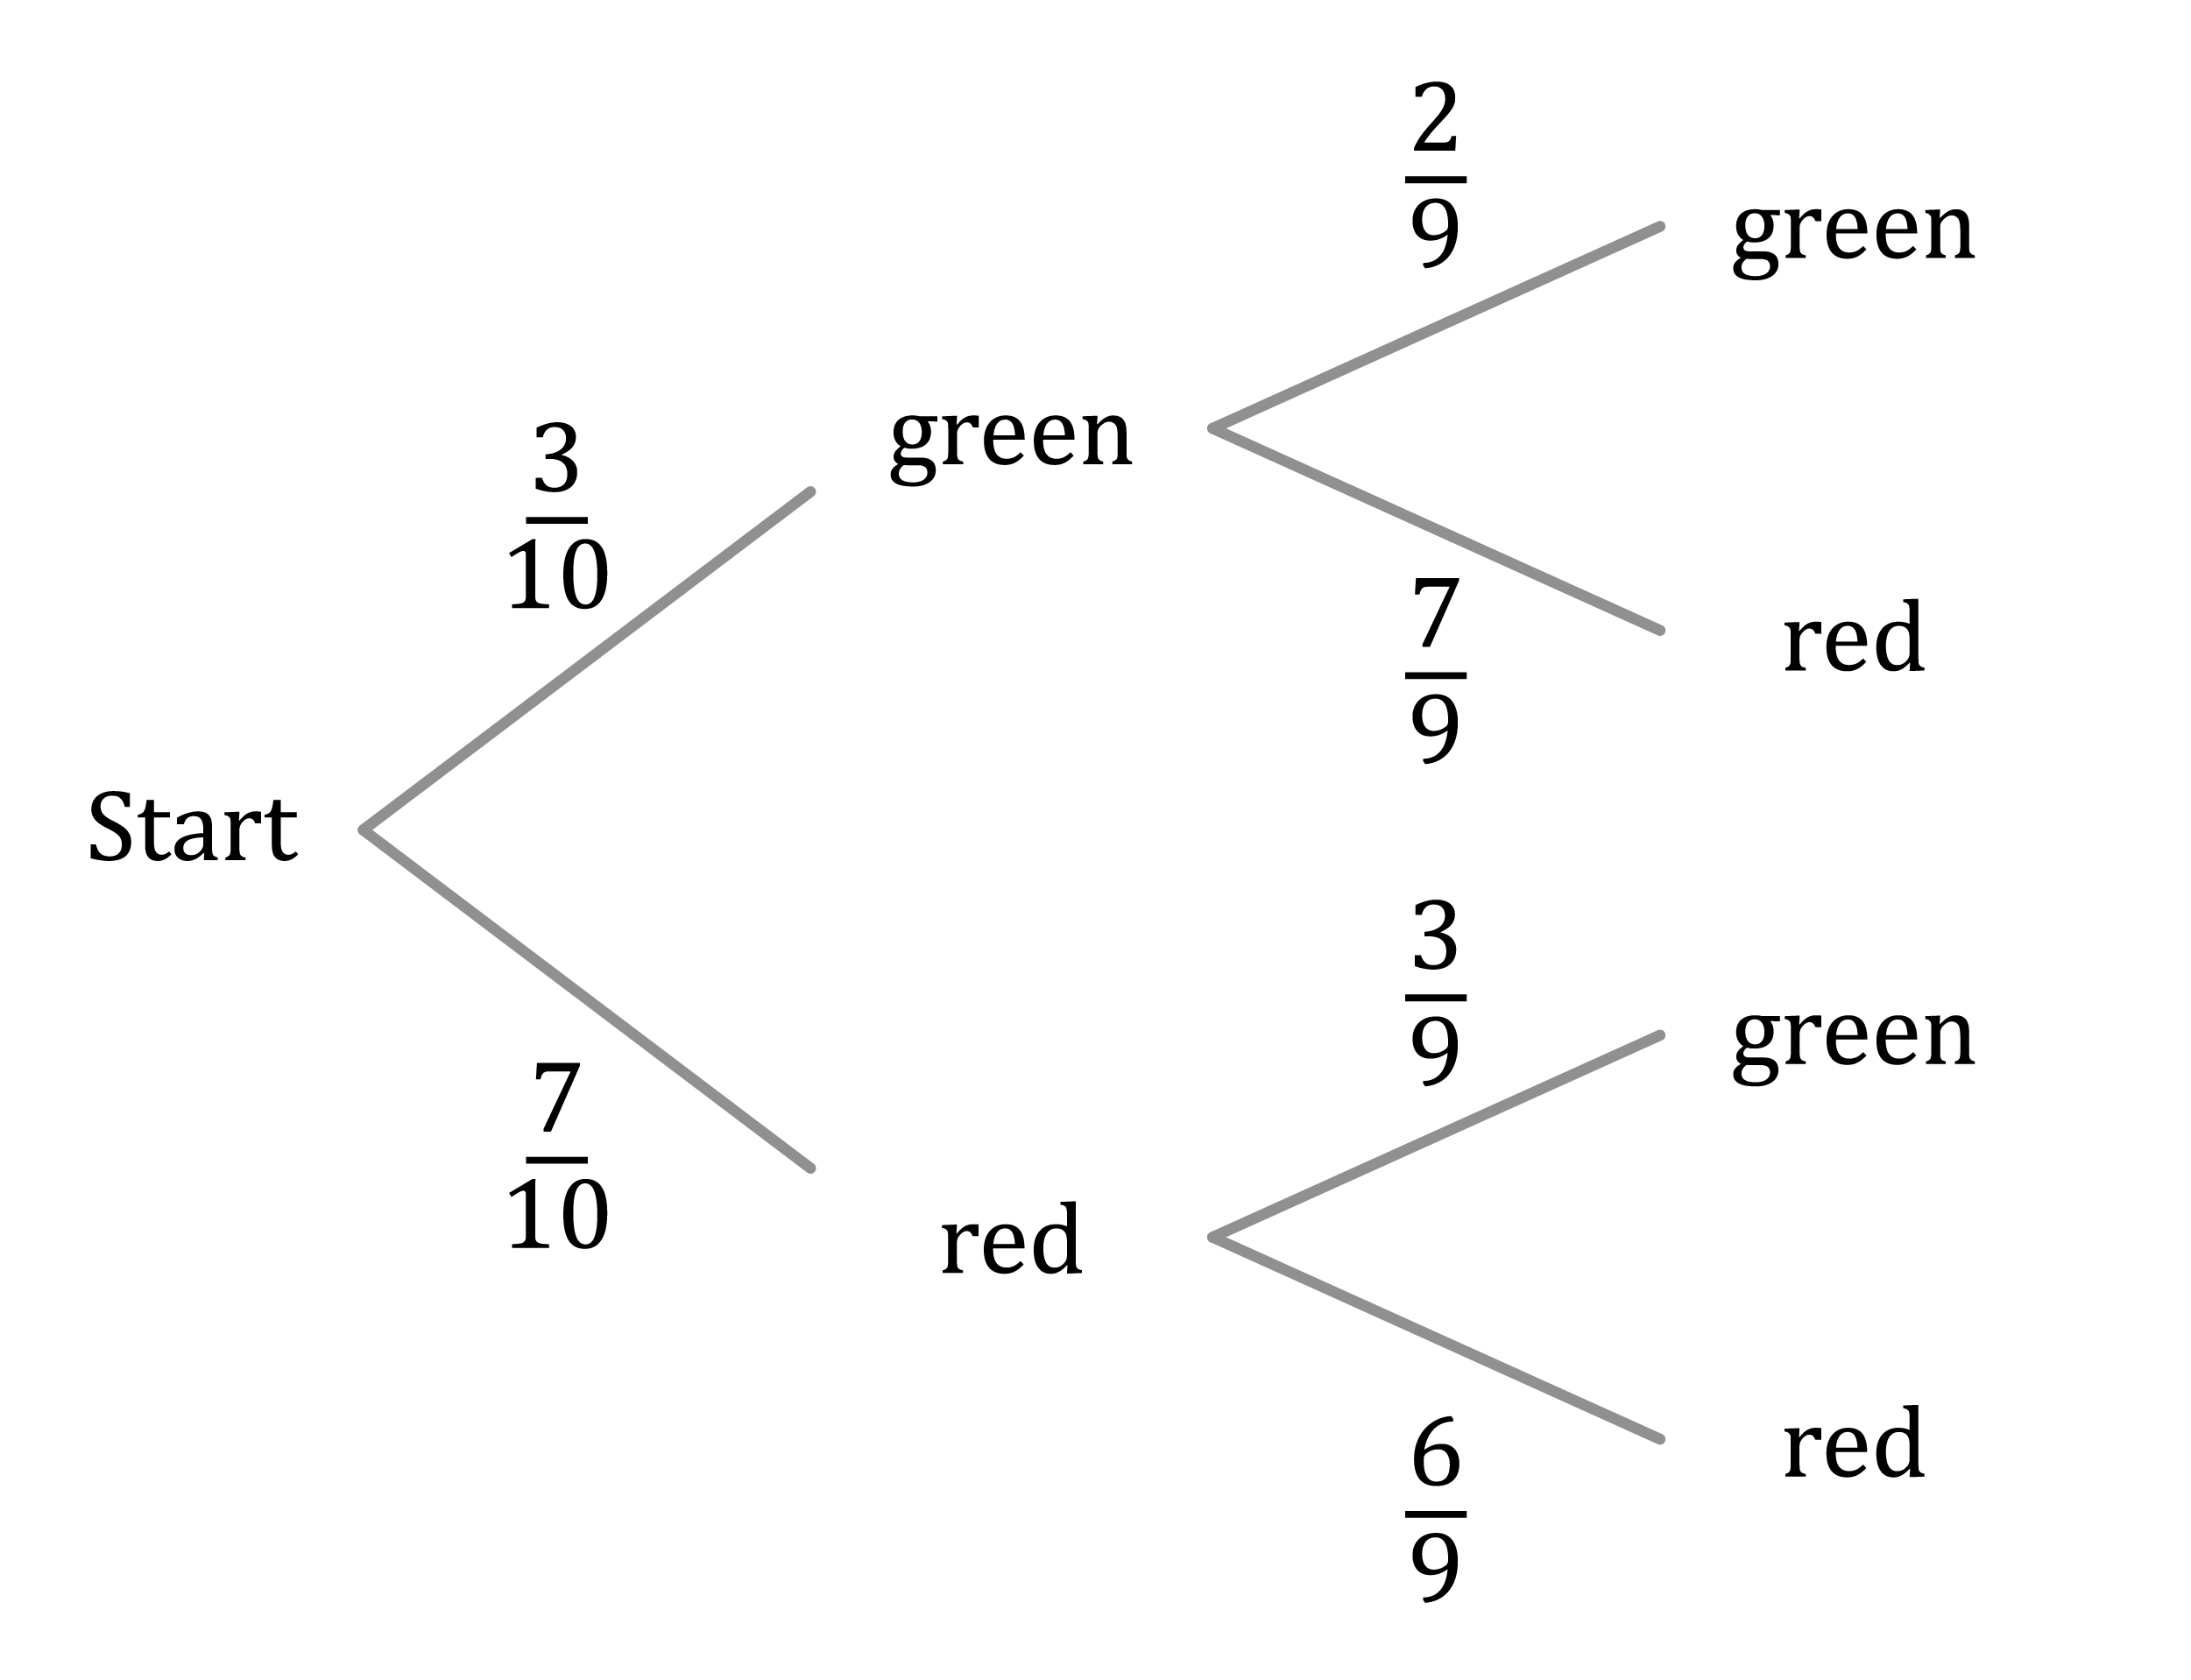
\includegraphics[scale=.06]{chance_tree}
\end{center}

\paragraph{Regola della catena} Per calcolare la probabilità di una qualsiasi foglia, che considero come una sequenza di esiti, bisogna individuare qual è il percorso che porta ad essa.
\begin{equation}
	P(\text{ramo}) = \text{prodotto delle probabilità dei sotto rami}
\end{equation}

\paragraph{Regola di fattorizzazione}
\begin{equation}
	P(\text{unione dei rami}) = \text{somma delle probabilità dei rami}
\end{equation}

\subsection{Indipendenza}
Vogliamo tradurre in linguaggio matematico il fatto che la probabilità di $B$ non cambia sapendo che accada $A$ e viceversa.
\begin{definition}
	Dati $n$ eventi $A_1, \ldots, A_n$, questi sono indipendenti se per ogni $k$ con $2 \leq k \leq n$ e per ogni scelta di interi $1 \leq i_1 < i_2< \ldots < i_k \leq n$ vale
	\begin{equation}
		\mathbb{P}(A_{i_1} \cap \ldots \cap A_{i_k}) = \mathbb{P}(A_{i_1}) \cdot  \ldots \cdot \mathbb{P}(A_{i_k})
	\end{equation}
\end{definition}

\begin{observation}
	Questa definizione equivale a dire che $P(A\vert B) = P(A)$ e $P(B \vert A) = P(B)$.
\end{observation}

\begin{observation}
	Se $P(A)=0$  oppure $P(A)=1$ allora $A$ è indipendente da qualsiasi altro evento.
\end{observation}

\begin{observation}
	Due eventi disgiunti non possono essere indipendenti a meno che uno dei due non sia trascurabile.
\end{observation}

\begin{observation}
	Due eventi possono essere indipendenti anche in presenza di una relazione causale. Viceversa due eventi possono essere dipendenti anche in assenza di una relazione causale.
\end{observation}

\subsubsection{Schema di Bernoulli}
Consideriamo $n$ prove ripetute di un esperimento in cui gli esiti sono successo, denominato come $1$ o insuccesso come $0$. Sia $p$ la probabilità di successo nella singola prova.
\begin{equation*}
	\Omega = \{(a_1, \ldots, a_n) \vert a_i \in \{0,1\}\} = \{0,1\}^n
\end{equation*}
Allora, visto che gli eventi sono indipendenti, la probabilità di una certa "stringa" (e.g. $(0,1,0)$) è:
\begin{align*}
	P(a_1, \ldots, a_n) & = P(a_1\text{ al 1° posto }) \cdot P(a_2\text{ al 2° posto }) \cdot \ldots \cdot P(a_n\text{ al n° posto }) \\
	& = p^{\#\text{ successi }} \cdot (1-p) ^ {\#\text{ insuccessi }} \\
	& = p^{\sum_{i=1}^{n}a_i} \cdot (1-p)^{n - \sum_{i=1}^{n}a_i} 
\end{align*}